\subsection{切面名称与弱目标统计}
\inputtable{tab13_views}


\paragraph{补充弱目标统计。}
完整 VCRE-Fib 在测试集上的框内平均响应、框外响应占比、框内/框外平均响应比分别为 0.570815、0.666595、359,012.493654；w/o View 对应为 0.499237、0.550558、1,678,411.504391。框外响应占比为目标框外注意力响应之和占总响应的比例。最后一项的分母截断于 $10^{-8}$，全视野框可产生很大比值。这些是描述性响应统计，并非定位准确性指标。表~\ref{tab:views} 比较两个含切面头模型的逐类召回率，评价产物另提供预测频率与混淆矩阵。

\subsection{病例选择与显示协议}\label{sec:appendix-case-protocol}
切面报告 accuracy/macro-F1，弱目标 Dice/IoU 使用阈值 0.5。从包含 12 个测试病例和 4 个验证病例的候选池中，选取覆盖四种真实切面的 4 个完整模型测试病例用于正文，另选两例验证病例用于附录。定位对应候选在切面内优先按弱框 Dice 选择。范围扩展候选要求框外响应占比 0.5--0.9、Dice 大于 0.1、阈值响应与框内相交，且至少 10\% 响应面积在全部显示框之外。各池内部按患者去重。三列使用相同处理后 ROI、固定 $[0,1]$ 定位色标、0.55 透明度和青色 0.5 轮廓。这些是筛选示例，当前不附加扩展区域的医生解释。

正文展示四个筛选的测试集病例。图~\ref{fig:valcases} 展示两例定位响应超出局部框的验证集病例，独立于测试集排名与空间指标；其中首例的预测切面与参考切面不同。
\begin{figure}[!htbp]
\centering
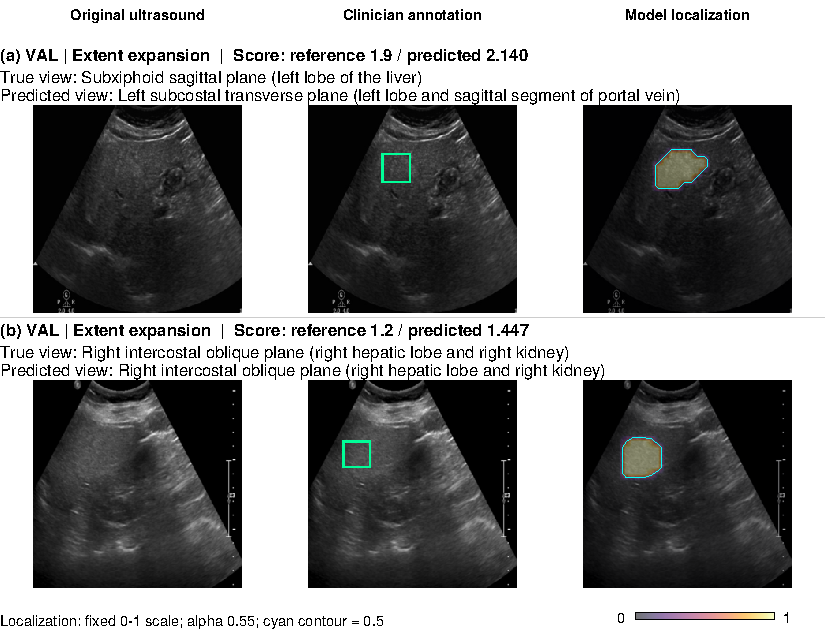
\includegraphics[width=\linewidth]{figures/assets/fig06_validation_cases.pdf}
\caption{定位响应超出局部框的验证集病例。预测使用参与定量评价的冻结检查点。三列依次呈现原始 ROI、医生标注与模型定位，文字标出参考及预测评分和扫查切面。首例的预测切面与参考切面不同。框外响应指出可供检查的位置，不表示已确定完整病灶范围。}
\label{fig:valcases}
\end{figure}
